% 2009 年广东卷（理科）第 18 题：棱长为 2 的正方体及其中的点 E、F、G。
% 来源 PDF：.work/ocr-local/sources/2009广东理.pdf
% SHA-256：5256b35235a042e254d36c111af3eda0f5dd8f552664021d0bace5c05582ad04
% 原页：第 2 页（A3 三栏）第 1 栏，印刷页 520。
% 绘制依据：斜二测式画法，前表面 A B B1 A1，纵深方向朝右上；D、C、D1、C1 为后表面
%   顶点。E 为正方形 BCC1B1 的中心，F 为 C1D1 中点，G 为 AA1 中点；E1、G1 分别是
%   E、G 在平面 DCC1D1 内的正投影（即 CC1、DD1 的中点）。
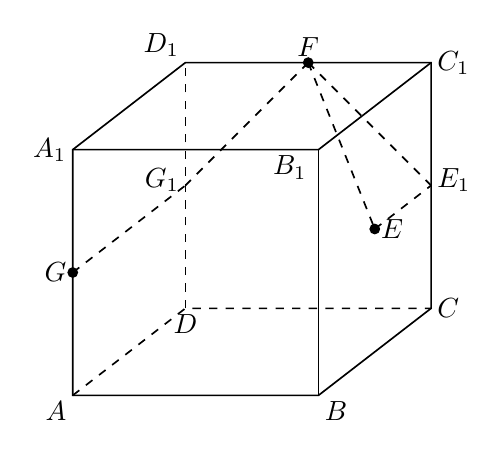
\begin{tikzpicture}[scale=1.3, semithick, every node/.style={inner sep=2pt}]

  \coordinate (A)  at (0,0);
  \coordinate (B)  at (2.4,0);
  \coordinate (A1) at (0,2.4);
  \coordinate (B1) at (2.4,2.4);
  \coordinate (D)  at (1.1,0.85);
  \coordinate (C)  at (3.5,0.85);
  \coordinate (D1) at (1.1,3.25);
  \coordinate (C1) at (3.5,3.25);
  \coordinate (E)  at (2.95,1.625);
  \coordinate (F)  at (2.3,3.25);
  \coordinate (G)  at (0,1.2);
  \coordinate (E1) at (3.5,2.05);
  \coordinate (G1) at (1.1,2.05);

  % 可见棱
  \draw (A) -- (B) -- (C) -- (C1) -- (D1) -- (A1) -- cycle;
  \draw (A1) -- (B1) -- (C1);
  \draw (B) -- (B1);

  % 不可见棱
  \draw[dashed] (A) -- (D) -- (C);
  \draw[dashed] (D) -- (D1);

  % 辅助线
  \draw[dashed] (F) -- (E);
  \draw[dashed] (F) -- (E1);
  \draw[dashed] (F) -- (G1);
  \draw[dashed] (E) -- (E1);
  \draw[dashed] (G) -- (G1);

  \fill (E) circle (1.5pt);
  \fill (F) circle (1.5pt);
  \fill (G) circle (1.5pt);

  \node[below left]  at (A)  {$A$};
  \node[below right] at (B)  {$B$};
  \node[right]       at (C)  {$C$};
  \node[below]       at (D)  {$D$};
  \node[left]        at (A1) {$A_1$};
  \node[below left, xshift=-2pt] at (B1) {$B_1$};
  \node[right]       at (C1) {$C_1$};
  \node[above left]  at (D1) {$D_1$};
  \node[right]       at (E)  {$E$};
  \node[above]       at (F)  {$F$};
  \node[left]        at (G)  {$G$};
  \node[right, yshift=2pt]  at (E1) {$E_1$};
  \node[left, yshift=2pt]   at (G1) {$G_1$};
\end{tikzpicture}
